\subsection{System Hardware}

The hardware setup combines mmWave radars, an inertial sensor, and auxiliary components into a compact test platform.  
In this section, we describe the role of each element, how they were mechanically integrated, and how the radar configuration was selected for odometry tasks.  

\vspace{0.5em}
\subsubsection{System Sensors}
\hfill
\\
The sensors that are implemented and used in this project are the following:
\vspace{0.5em}
\subsubsubsection{mmWave Radar (IWR6843AOP)}
\hfill
\\
\indent The IWR6843AOPEVM development board from Texas Instruments features the IWR6843AOP, a high performance 4D mmWave FMCW sensor with Antenna On Package (AOP) design.
Although IWR6843AOP is intended for industrial applications and its complementary chip, AWR6843AOP, for automotive applications, IWR6843AOP was used in this project because it is available in the form of this development board and the two chips are identical in terms of their functionalities, only differing in compliance with automotive  industry \cite{iwr_awr_diff}.
Its small physical size, due to its AOP design, makes it an optimal choice for the desired mounting position, the go-kart's steering column.
\begin{figure}[!htbp]
    \centering
    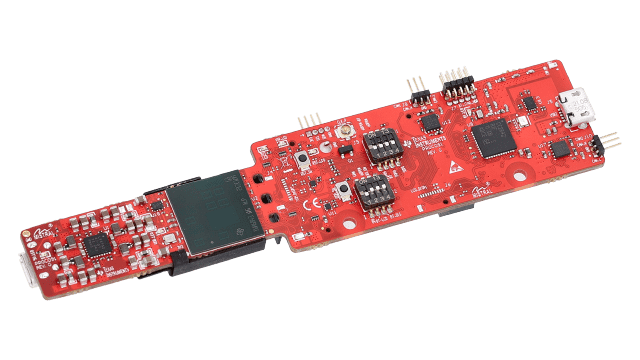
\includegraphics[width=0.7\linewidth]{images/iwr6843aopevm-angled.png}
    \caption{IWR6843AOP sensor\\
    \textit{Source: Texas Instruments, available at \href {https://www.ti.com/content/dam/ticom/images/products/ic/processors/evm-boards/iwr6843aopevm-angled.png}{https://www.ti.com/tool/IWR6843AOPEVM}}}
    \label{fig:IWR6843AOP sensor}
\end{figure}

\par
The IWR6843AOP radar sensor operates within the frequency range of \SIrange{60}{64}{\giga\hertz} and integrates 4 receive (RX) and 3 transmit (TX) antennas, radio frequency (RF) front-end stages, analog signal processing, and digital signal processing (DSP).
It offers a wide range of communication interfaces including SPI, I2C, CAN-FD, UART and LVDS for raw data access and an Arm Cortex-R4F microcontroller for user-applications as shown in the Figure~\ref{fig:IWR6843AOP_internal} \cite{dev_board_page}.

\begin{figure}[!htbp]
    \centering
    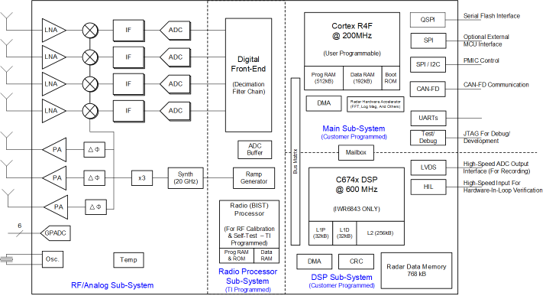
\includegraphics[width=1.0\linewidth]{images/blockdiagram.png}
    \caption{IWR6843AOP functional block diagram.\\
    \textit{Source: Texas Instruments, available at \url{https://www.ti.com/ds_dgm/images/fbd_swrs219f.gif}}}
    \label{fig:IWR6843AOP_internal}
\end{figure}

\begin{comment}
    Here create a connecto to the calibration of the sensor
\end{comment}

As some operating parameters influence each other, their selection must be done carefully while observing the influence of the trade-offs involved.
This could be referred to as "sensor tuning" and is a critical step because it directly impacts the system's accuracy and performance.

The following operating parameters can be tuned:
\begin{itemize}
    \item Frame rate
    \item Range resolution
    \item Maximum unambigious range
    \item Maximum radial velocity
    \item Radial velocity resolution
\end{itemize}

Tuning these operating parameters introduces trade-offs by influencing each other in the following ways:
\begin{table}[h]
    \centering
    \resizebox{\columnwidth}{!}{
    \begin{tabular}{|l|l|p{3.5cm}|p{3.5cm}|p{3.5cm}|}
        \hline
        \textbf{Tuning Parameter} & \textbf{Effect on Performance} & \textbf{Related HW Block} & \textbf{Trade-Off} \\
        \hline
        Frame Rate & Higher FPS = faster updates but more processing load & C674x DSP, Radar Data Memory & Higher FPS reduces maximum range \\
        \hline
        Range Resolution & Higher resolution = better object separation & ADC, 1D FFT (Range FFT) & Higher resolution reduces max range \\
        \hline
        Maximum Range & Determines farthest detectable object & RF Front-End, PA, LNA, ADC & Higher range lowers resolution \\
        \hline
        Radial Velocity Resolution & Improves speed accuracy & DSP, 2D FFT (Doppler FFT) & Higher resolution requires more chirps \\
        \hline
        Maximum Radial Velocity & Detects fast-moving objects & Chirp rate, TX Antennas, 2D FFT & Higher max velocity reduces resolution \\
        \hline
    \end{tabular}
    }
    \caption{Radar System Tuning Parameters and Trade-offs}
    \label{tab:mmWave_Sensor_Parameters}
\end{table}
The resulting overall accuracy of the velocity and distance measurements is again dependent on these operating parameters:
\begin{itemize}
\item \textbf{Radial velocity accuracy:} A fine balance between velocity resolution and frame rate must be maintained to ensure precise Doppler shift measurements. Lower resolution results in rounded velocity values, while an excessively high frame rate may introduce computational bottlenecks.
\item \textbf{Distance accuracy:} Optimizing range resolution and maximum range ensures that detected objects are positioned accurately within the environment. Increasing range often sacrifices resolution, leading to potential inaccuracies in close-range detections.
\item \textbf{Signal processing considerations:} The FFT calculation parameters directly affect both range and Doppler calculations, influencing the ability to distinguish between objects and detect small velocity variations.
\end{itemize}
\vspace{0.5em}
\subsubsubsection{Inertial Measurement Unit (IMU)}  
\hfill
\\
\indent The MTi-G-710 from Xsens is a high-performance GNSS/INS module that integrates a 3D accelerometer, 3D gyroscope, 3D magnetometer, and barometer with an onboard GNSS receiver.  
Although designed as a complete navigation unit capable of delivering position and velocity estimates, in this project it was used specifically for its orientation outputs, provided in the form of quaternions, Euler angles, or rotation matrices \cite{mti710_manual}.  
Its compact form factor and proven sensor-fusion engine made it a suitable choice for integration into the test platform, complementing the radar subsystem by supplying real-time orientation references.  

For the present setup, the device was configured to output quaternions, as this representation avoids singularities inherent in Euler angles and provides numerical stability for continuous tracking.  
These quaternions were used to track the vehicle attitude and to align radar point clouds within a consistent vehicle-centric coordinate frame.  
By relying on the MTi-G-710 internal fusion engine rather than implementing custom filtering, the system leveraged factory-calibrated algorithms for bias correction and drift reduction, minimizing processing overhead on the host platform.  

To interface with the device and parse its MTData2 protocol, an open-source implementation from Scottapotamas was adopted \cite{xsens_repo}.  
This repository enabled robust packet parsing and quaternion extraction in Python, ensuring seamless integration of the IMU data stream into the radar processing pipeline.  

\begin{figure}[!htbp]
    \centering
    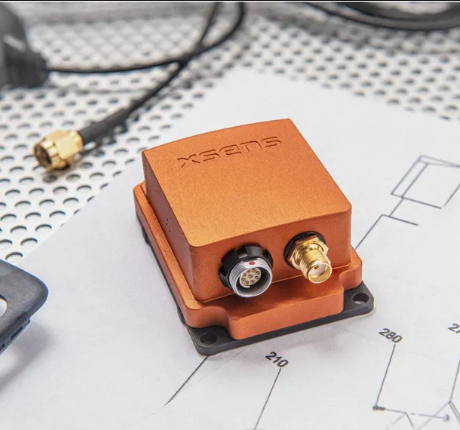
\includegraphics[width=0.65\linewidth]{images/mti_g710.png}
    \caption{MTi-G710 high-performance inertial navigation system (INS).\\
    \textit{Source: Movella, available at \url{https://www.movella.com/sensor-modules/xsens-mti-7-gnss-ins}}}
    \label{fig:MTi-G710 sensor}
\end{figure}

\subsubsubsection{Webcam}
\hfill
\\
\indent A Logitech C270 HD webcam was included in the experimental platform for the sole purpose of video recording.  
Unlike the radar and IMU, the camera was not integrated into the sensing or processing pipeline and did not contribute any data to the odometry estimation system.  
Its role was limited to providing visual documentation of the test environment, allowing experiments to be reviewed and contextualized with synchronized video footage.  
